\documentclass[a4paper,12pt]{ctexart}

\usepackage[left=2.3cm,right=2.3cm,top=2.7cm,bottom=2.7cm]{geometry}
\usepackage{graphicx}
\usepackage{xcolor}
\usepackage{float}
\usepackage{booktabs}
\usepackage{array}
\usepackage{amsmath,amssymb,bm}
\usepackage{fancyhdr}
\usepackage{lastpage}
\usepackage{hyperref}
\usepackage{pgfplots}
\usepackage{listings}
\usepackage{algorithm}
\usepackage{algorithmicx}
\usepackage{algpseudocode}

\pgfplotsset{compat=1.18}

\hypersetup{
    colorlinks=true,
    linkcolor=black,
    urlcolor=blue,
    citecolor=black
}

\lstset{
    language=C++,
    breaklines=true,
    basicstyle=\small\ttfamily,
    keywordstyle=\color{blue!70}\bfseries,
    commentstyle=\color{green!40!black},
    stringstyle=\color{red!60!black},
    numbers=left,
    numberstyle=\tiny\color{blue!50},
    frame=single,
    columns=flexible,
    showstringspaces=false
}

\floatname{algorithm}{Algorithm}
\renewcommand{\algorithmicrequire}{\textbf{Input:}}
\renewcommand{\algorithmicensure}{\textbf{Output:}}
\renewcommand{\contentsname}{目录}
\renewcommand{\refname}{参考文献}
\renewcommand{\figurename}{图}
\renewcommand{\tablename}{表}
\renewcommand{\today}{\number\year 年 \number\month 月 \number\day 日}

\makeatletter
\newenvironment{breakablealgorithm}
  {
   \begin{center}
     \refstepcounter{algorithm}
     \hrule height .8pt depth 0pt \kern 2pt
     \renewcommand{\caption}[2][\relax]{
       {\raggedright\textbf{\ALG@name~\thealgorithm} ##2\par}
       \ifx\relax##1\relax
         \addcontentsline{loa}{algorithm}{\protect\numberline{\thealgorithm}##2}
       \else
         \addcontentsline{loa}{algorithm}{\protect\numberline{\thealgorithm}##1}
       \fi
       \kern2pt\hrule\kern2pt
     }
  }
  {
     \kern2pt\hrule\relax
   \end{center}
  }
\makeatother

\pagestyle{fancy}
\fancyhf{}
\lhead{\kaishu \leftmark}
\rhead{\kaishu 并行程序设计实验报告}
\cfoot{\thepage\ / \pageref{LastPage}}
\renewcommand{\headrulewidth}{0.1pt}
\renewcommand{\footrulewidth}{0pt}
\setcounter{tocdepth}{2}

\begin{document}

\begin{titlepage}
    \begin{center}
        
\includegraphics[width=0.8\textwidth]{assets/NKU.png}\\[1cm]

        \vspace{20mm}

        {\huge\bfseries\kaishu 计算机学院\par}
        \vspace{0.5cm}
        {\huge\bfseries\kaishu 并行程序设计实验报告\par}
        \vspace{2.3cm}
        {\Huge\bfseries\kaishu NTT 的 SIMD 向量化优化实验\par}

        \vspace{\fill}

        {\LARGE\kaishu 姓名：马禹翔\par}
        \vspace{0.5cm}
        {\LARGE\kaishu 学号：2410933\par}
        \vspace{0.5cm}
        {\LARGE\kaishu 专业：计算机科学与技术\par}

        \vfill
        {\Large \today\par}
    \end{center}
\end{titlepage}

\tableofcontents
\thispagestyle{plain}
\clearpage

\section*{代码仓库说明}

本实验完整源码已上传至 GitHub，访问地址如下：

\begin{center}
\url{https://github.com/s1nk141/nku26}
\end{center}

\section{实验目的}

本实验围绕 NTT的 SIMD 优化展开。NTT 常用于多项式乘法、大整数乘法以及卷积计算，其核心计算过程具有规则的蝶形结构，适合利用 SIMD 指令进行向量化。实验目标如下：

\begin{enumerate}
  \item 理解 NTT 与快速傅里叶变换类似的分治蝶形计算结构；
  \item 掌握模意义下加法、减法、乘法在 NTT 中的作用；
  \item 实现普通串行 NTT 与 AVX2 SIMD 优化版本，并验证二者结果一致；
  \item 探索 SIMD 向量化取模和向量化蝶形变换的实现方式；
  \item 通过不同问题规模下的实验数据分析 SIMD 优化对 NTT 性能的影响。
\end{enumerate}

\section{实验原理}

\subsection{NTT 问题描述}

给定两个多项式：

\begin{equation}
A(x)=\sum_{i=0}^{n-1}a_i x^i,\quad B(x)=\sum_{i=0}^{n-1}b_i x^i
\end{equation}

多项式乘法的结果为：

\begin{equation}
C(x)=A(x)B(x)
\end{equation}

如果直接计算卷积，则需要 $O(n^2)$ 次乘加操作。当 $n$ 较大时开销很高，而NTT 将多项式转换到模数域下的点值表示，在点值域中逐点相乘，再通过逆变换恢复系数，从而将复杂度降低到：

\begin{equation}
O(n\log n)
\end{equation}

\subsection{模数与原根选择}
最开始尝试直接使用常见模数 998244353，但在 SIMD 版本中使用 double 近似取模时出现了与串行结果不一致的问题。检查后发现两个模数域元素相乘的结果接近 $10^{18}$，超过 double 能够精确表示整数的范围。

故我们选择如下 NTT 友好素数：

\begin{equation}
p=7340033=7\times 2^{20}+1
\end{equation}

其原根取：

\begin{equation}
g=3
\end{equation}

7340033满足 $p-1$ 含有较大的 $2$ 的幂因子，因此可以支持长度不超过 $2^{20}$ 的二次幂 NTT。同时，7340033还满足两个模数域元素相乘后落在 double 精确整数表示范围内，故可以用 AVX2 的 double 向量实现近似除法取模而不破坏本实验规模下的正确性。

\subsection{蝶形变换}

NTT 的核心为蝶形变换。设当前步长为 $mid$，旋转因子为 $w$，则一次蝶形计算为：

\begin{equation}
u=a[i+j],\quad v=a[i+j+mid]\cdot w \bmod p
\end{equation}

\begin{equation}
a[i+j]=(u+v)\bmod p
\end{equation}

\begin{equation}
a[i+j+mid]=(u-v+p)\bmod p
\end{equation}

同一层中不同 $j$ 位置的蝶形计算彼此独立，因此可以把连续若干个 $j$ 同时放入 SIMD 寄存器中计算。本实验每次处理 4 个 double 通道，对应 4 组蝶形操作。

\subsection{向量化取模}

AVX2 对 32 位整数乘法与 64 位取模的支持并不如浮点运算直接，因此我们采用浮点数近似取模策略。对于乘积 $x=a\cdot b$，有：

\begin{equation}
x\bmod p=x-\left\lfloor \frac{x}{p}\right\rfloor p
\end{equation}

在实现时将 4 个乘积放入 \texttt{\_\_m256d}，使用 \texttt{\_mm256\_floor\_pd} 得到商，再减去商与模数的乘积。由于选择的模数较小，乘积仍可被 double 精确表示，因此实验中 SIMD 版本与串行版本保持完全一致。

\section{实验平台与实验方案}

\subsection{实验平台}

本实验在 Windows 环境下完成，采用 C++ 编写程序，使用 g++ 编译，并通过 AVX2 intrinsics 实现 SIMD 优化。实验平台配置如下：

操作系统：Windows

编译器：g++ 10.3.0

编译选项：\texttt{-O2 -mavx2 -std=c++17}

SIMD 指令集：AVX2

\subsection{测试数据设计}

程序使用固定随机种子生成多项式系数：

\begin{equation}
a_i,b_i\in[0,p)
\end{equation}

每组输入分别调用串行 NTT 卷积和 AVX2 NTT 卷积，并逐项比较结果。只有当所有系数完全一致时，才认为该规模测试通过正确性验证。

\subsection{测试规模设计}

选取如下多项式长度进行测试：

\begin{enumerate}
  \item $n=1024$
  \item $n=4096$
  \item $n=16384$
  \item $n=65536$
  \item $n=262144$
\end{enumerate}


\subsection{计时方法}

实验采用 \texttt{chrono::high\_resolution\_clock} 计时，单位为微秒。为减少单次运行波动，小规模测试重复 10 次，中等规模重复 5 次，大规模重复 3 次，并取平均值作为最终时间。

\section{算法设计与代码实现}

\subsection{算法思路说明}

本实验共实现两类算法：

\begin{enumerate}
  \item \textbf{串行 NTT}：使用普通循环完成位逆序置换、蝶形变换、点值乘法和逆变换；
  \item \textbf{AVX2 NTT}：保留位逆序置换为串行过程，将蝶形变换、模乘和逆变换末尾的乘法归一化进行 SIMD 向量化。
\end{enumerate}

其中位逆序置换的数据访问不连续，很难高效向量化；而每一层内部的蝶形计算结构规则、不存在交叉依赖，是本实验主要优化对象。

\subsection{核心代码}

下面是 SIMD 模乘的核心代码。一次处理 4 个模乘，并将各类运算与边界修正都放在向量寄存器中完成。

\begin{lstlisting}[title=AVX2 向量化模乘]
__m256d mul_mod_pd(__m256d x, __m256d y) {
    __m256d prod = _mm256_mul_pd(x, y);
    __m256d q = _mm256_floor_pd(
        _mm256_mul_pd(prod, _mm256_set1_pd(INV_MOD_D)));
    __m256d r = _mm256_sub_pd(
        prod, _mm256_mul_pd(q, _mm256_set1_pd(MOD_D)));
    __m256d ge = _mm256_cmp_pd(r, _mm256_set1_pd(MOD_D), _CMP_GE_OQ);
    r = _mm256_sub_pd(r, _mm256_and_pd(ge, _mm256_set1_pd(MOD_D)));
    __m256d lt = _mm256_cmp_pd(r, _mm256_setzero_pd(), _CMP_LT_OQ);
    r = _mm256_add_pd(r, _mm256_and_pd(lt, _mm256_set1_pd(MOD_D)));
    return r;
}
\end{lstlisting}

下面是 AVX2 蝶形变换的关键部分。程序每次取 4 个连续的 $u$、4 个连续的待乘元素以及 4 个对应旋转因子，完成 4 组蝶形运算。

\begin{lstlisting}[title=AVX2 蝶形变换核心]
for (; j + 4 <= mid; j += 4) {
    int ws[4];
    ws[0] = w;
    ws[1] = scalar_mul_mod(ws[0], wlen);
    ws[2] = scalar_mul_mod(ws[1], wlen);
    ws[3] = scalar_mul_mod(ws[2], wlen);
    w = scalar_mul_mod(ws[3], wlen);

    __m256d u = _mm256_set_pd(a[i + j + 3], a[i + j + 2],
                              a[i + j + 1], a[i + j]);
    __m256d t = _mm256_set_pd(a[i + j + mid + 3],
                              a[i + j + mid + 2],
                              a[i + j + mid + 1],
                              a[i + j + mid]);
    __m256d ww = _mm256_set_pd(ws[3], ws[2], ws[1], ws[0]);
    __m256d v = mul_mod_pd(t, ww);

    __m256d add = _mm256_add_pd(u, v);
    __m256d sub = _mm256_sub_pd(u, v);
    // 后续通过比较掩码修正 add >= MOD 和 sub < 0 的情况
}
\end{lstlisting}

\subsection{伪代码描述}

\begin{breakablealgorithm}
\caption{AVX2 优化的 NTT 卷积}
\begin{algorithmic}[1]
\Require 多项式系数数组 $A,B$
\Ensure 卷积结果 $C$
\State 将数组长度扩展为二次幂 $n$
\State 对 $A$ 执行 AVX2-NTT
\State 对 $B$ 执行 AVX2-NTT
\For{$i=0$ to $n-1$ step 4}
    \State 使用 AVX2 同时计算四个 $A[i]\gets A[i]\cdot B[i]\bmod p$
\EndFor
\State 对 $A$ 执行 AVX2 逆 NTT
\State 截取前 $|A|+|B|-1$ 项作为卷积结果
\end{algorithmic}
\end{breakablealgorithm}

\section{实验结果}


\begin{table}[H]
\centering
\begin{tabular}{ccccc}
\toprule
$n$ & 串行 NTT($\mu s$) & AVX2 NTT($\mu s$) & 加速比 & 正确性 \\
\midrule
1024   & 297.700    & 200.500    & 1.485 & yes \\
4096   & 1818.200   & 1157.700   & 1.571 & yes \\
16384  & 7498.400   & 5629.600   & 1.332 & yes \\
65536  & 32516.000  & 26409.000  & 1.231 & yes \\
262144 & 158737.667 & 124178.333 & 1.278 & yes \\
\bottomrule
\end{tabular}
\caption{不同规模下串行 NTT 与 AVX2 NTT 性能对比}
\label{table:result}
\end{table}

\begin{figure}[H]
\centering
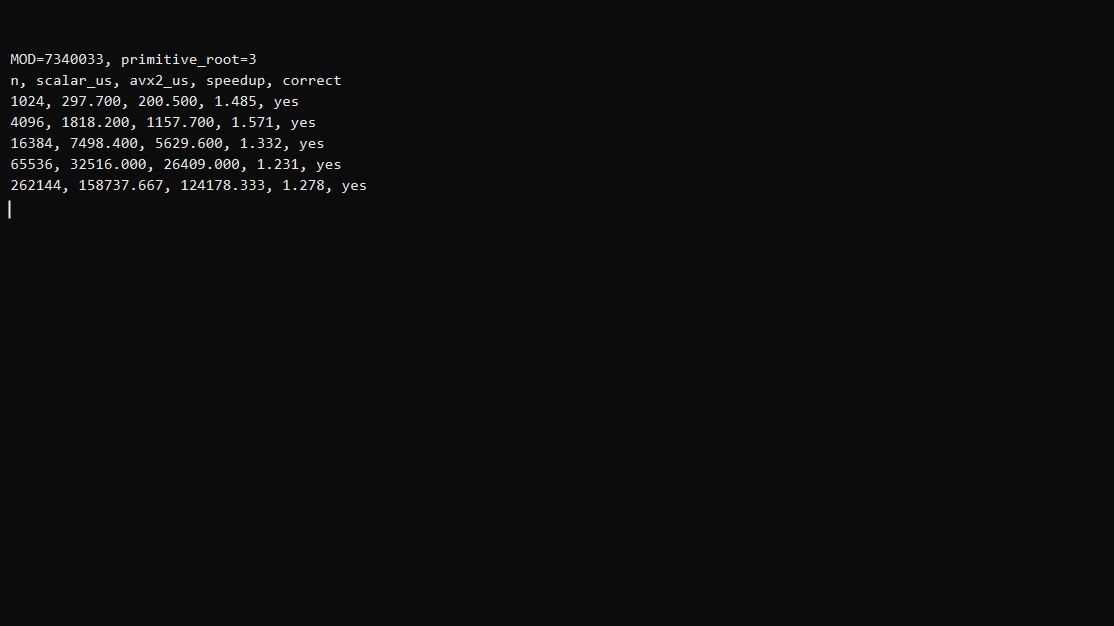
\includegraphics[width=0.86\textwidth]{assets/local_result.png}
\caption{本地 AVX2 NTT 测试结果截图}
\label{fig:local-result}
\end{figure}

\begin{figure}[H]
\centering
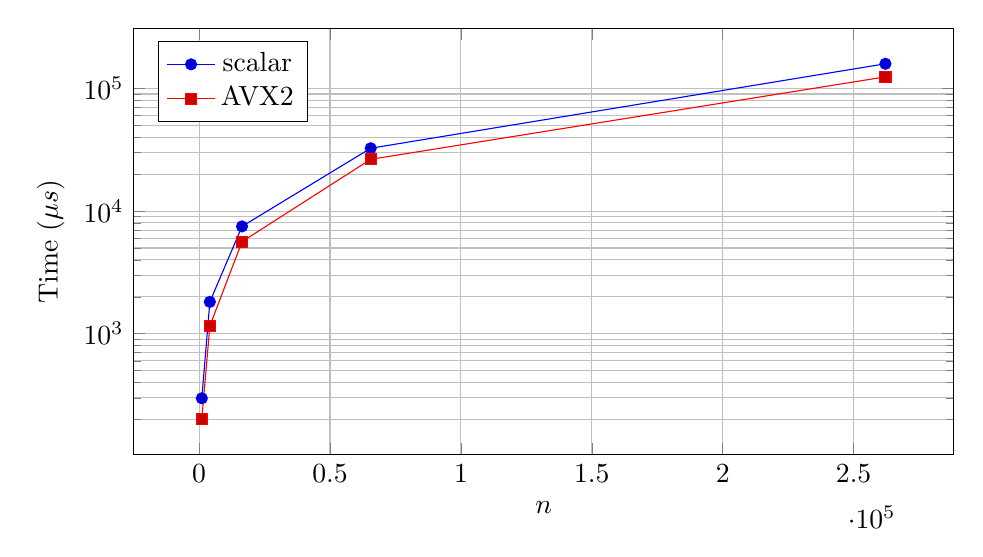
\begin{tikzpicture}
\begin{axis}[
    xlabel={$n$},
    ylabel={Time ($\mu s$)},
    ymode=log,
    log basis y={10},
    legend pos=north west,
    grid=both,
    width=12cm,
    height=7cm
]
\addplot coordinates {
(1024,297.700)
(4096,1818.200)
(16384,7498.400)
(65536,32516.000)
(262144,158737.667)
};
\addlegendentry{scalar}
\addplot coordinates {
(1024,200.500)
(4096,1157.700)
(16384,5629.600)
(65536,26409.000)
(262144,124178.333)
};
\addlegendentry{AVX2}
\end{axis}
\end{tikzpicture}
\caption{串行 NTT 与 AVX2 NTT 运行时间对比}
\end{figure}

\begin{figure}[H]
\centering
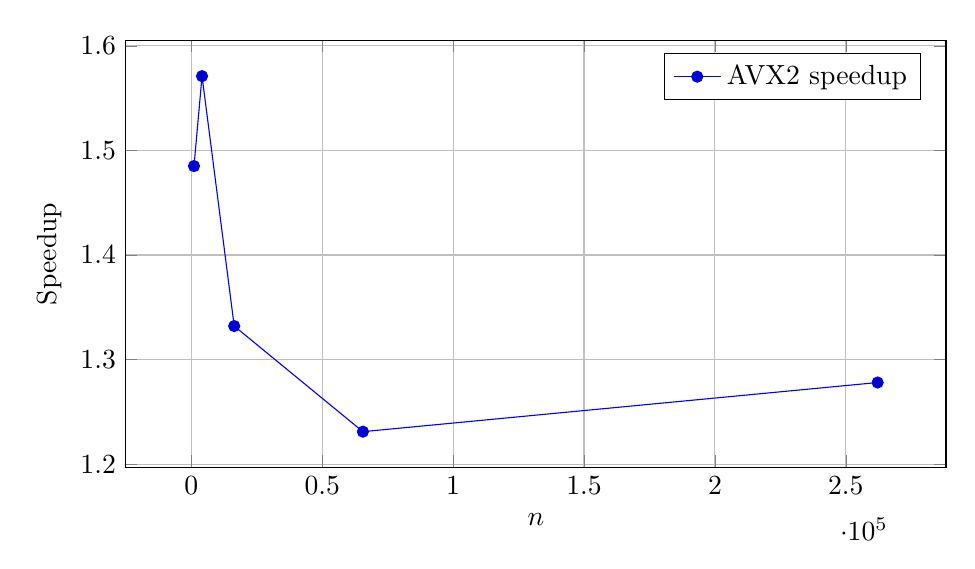
\begin{tikzpicture}
\begin{axis}[
    xlabel={$n$},
    ylabel={Speedup},
    grid=both,
    width=12cm,
    height=7cm,
    legend pos=north east
]
\addplot coordinates {
(1024,1.485)
(4096,1.571)
(16384,1.332)
(65536,1.231)
(262144,1.278)
};
\addlegendentry{AVX2 speedup}
\end{axis}
\end{tikzpicture}
\caption{AVX2 NTT 加速比变化}
\end{figure}

可以看出，AVX2 版本在所有测试规模下均通过正确性验证，并且整体速度快于串行版本。加速比处于 $1.23$ 到 $1.57$ 之间，说明向量化蝶形变换和向量化模乘确实起到了加速作用；而由于旋转因子递推、位逆序置换以及访存写回等，加速效果仍存在优化空间。

\subsection{ssh平台正确性验证}

如图所示，在远程 SSH 环境中运行 \texttt{test.sh} 脚本，同样可以验证程序正确性。

\begin{figure}[H]
\centering
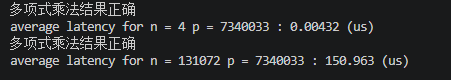
\includegraphics[width=0.72\textwidth]{assets/ssh_result.png}
\caption{远程 SSH 平台运行结果}
\label{fig:ssh-result}
\end{figure}

\section{汇编代码分析}

为了确认 SIMD 代码确实被编译为 AVX2 指令，本实验使用如下命令生成汇编代码：

\begin{lstlisting}[language=bash]
g++ -O2 -mavx2 -std=c++17 -S main.cc -o main_avx2.s
\end{lstlisting}

在生成的 \texttt{main\_avx2.s} 中，\texttt{mul\_mod\_pd} 函数和 \texttt{ntt\_avx2} 函数均出现了明显的 AVX2 向量指令。截取其中一段如下：

\begin{lstlisting}[language={[x86masm]Assembler}, title=AVX2 模乘相关汇编片段]
vmulpd   %ymm0, %ymm1, %ymm0
vmulpd   %ymm6, %ymm0, %ymm1
vroundpd $1, %ymm1, %ymm1
vmulpd   %ymm4, %ymm1, %ymm1
vsubpd   %ymm1, %ymm0, %ymm0
vcmppd   $29, %ymm4, %ymm0, %ymm1
vandpd   %ymm4, %ymm1, %ymm1
vsubpd   %ymm1, %ymm0, %ymm0
vaddpd   %ymm1, %ymm0, %ymm0
\end{lstlisting}

其中 \texttt{vmulpd} 对应 4 路 double 乘法，\texttt{vroundpd} 用于计算近似商的向下取整，\texttt{vsubpd} 用于完成 $x-\lfloor x/p\rfloor p$，\texttt{vcmppd} 与 \texttt{vandpd} 用于生成掩码并修正结果范围。该指令序列与源代码中的 \texttt{mul\_mod\_pd} 完全对应，说明向量化取模真正落到了SIMD 指令上。

在 \texttt{ntt\_avx2} 的蝶形计算部分，还可以观察到如下指令：

\begin{lstlisting}[language={[x86masm]Assembler}, title=AVX2 蝶形加减相关汇编片段]
vaddpd   %ymm0, %ymm7, %ymm8
vsubpd   %ymm0, %ymm7, %ymm1
vcmppd   $29, %ymm4, %ymm8, %ymm9
vcmppd   $17, %ymm5, %ymm1, %ymm0
vsubpd   %ymm9, %ymm8, %ymm8
vaddpd   %ymm1, %ymm0, %ymm0
\end{lstlisting}

这段代码对应 4 组蝶形变换中的加法分支和减法分支。由于 NTT 的每层蝶形操作内部没有跨元素依赖，编译后能够稳定形成以 \texttt{ymm} 寄存器为核心的向量计算序列。

\section{VTune 性能剖析}

为了进一步观察程序运行时的热点分布，我们使用VTune对 \texttt{ntt\_lab2.exe} 进行了 Hotspots 分析。图 \ref{fig:vtune-summary} 为 VTune Summary 页面截图，可以看到本次采集的 Elapsed Time 为 1.599 s，CPU Time 为 1.548 s，Total Thread Count 为 1，Parallelism 为 3.0\%。

\begin{figure}[H]
\centering
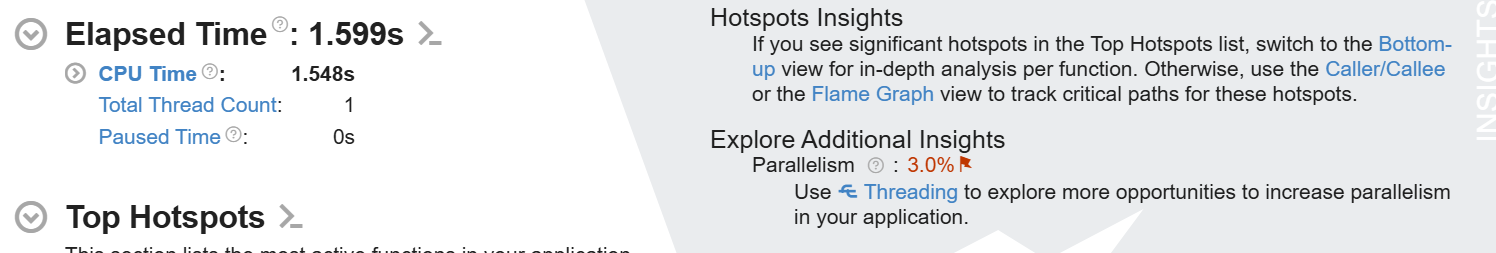
\includegraphics[width=0.95\textwidth]{assets/vtune_summary.png}
\caption{VTune Hotspots Summary 页面}
\label{fig:vtune-summary}
\end{figure}

CPU Time 与 Elapsed Time 非常接近，说明程序主要处于 CPU 计算状态，运行过程中没有明显的 I/O 等待或长时间阻塞。线程数为 1，Parallelism 为 3.0\%，表明程序运行在单线程上进行了simd优化，而不是多个cpu核心同时执行。

图 \ref{fig:vtune-hotspots} 给出了 VTune 的 Top Hotspots 结果。前两个位于 \texttt{ntt\_lab2.exe} 内部的函数分别占用 56.7\% 和 40.5\% 的 CPU Time，是主要性能瓶颈。

\begin{figure}[H]
\centering
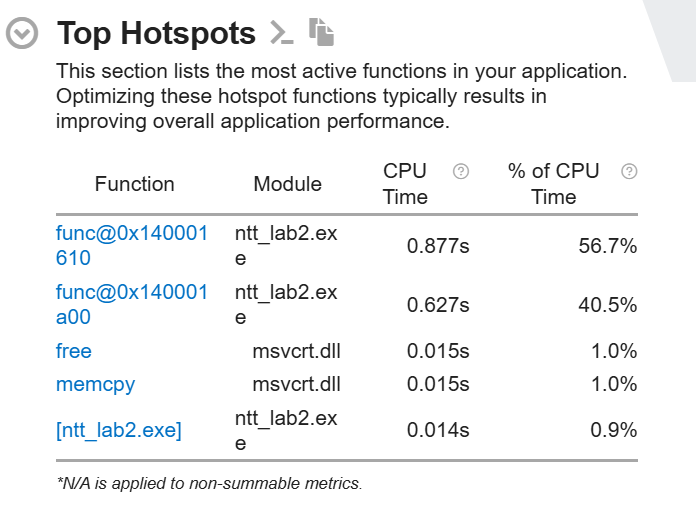
\includegraphics[width=0.68\textwidth]{assets/vtune_hotspots.png}
\caption{VTune Top Hotspots 页面}
\label{fig:vtune-hotspots}
\end{figure}

上述热点主要对应 NTT 变换、逆变换以及卷积过程中的核心计算循环。这一点与前文实验现象一致：NTT 的主要耗时集中在大量重复的蝶形计算和模乘操作中。因此，使用 AVX2 对这些核心循环进行向量化是合理的优化方向。另一方面，由于程序仍为单线程实现，VTune 的 CPU 利用率结果也解释了 Parallelism 较低的原因。
\section{实验过程中遇到的问题与解决方法}

\subsection{直接使用大模数导致浮点取模风险}

NTT 常用模数为 $998244353$。如果直接使用该模数，两个模数域元素相乘可达到约 $10^{18}$，超过 double 精确表示整数的范围，浮点近似取模容易产生错误。因此选择 $7340033$ 作为模数，使乘积保持在 double 可精确表示范围内，从而兼顾 SIMD 实现便利性与结果正确性。

\subsection{旋转因子生成仍有串行开销}

在实现 AVX2 蝶形计算时，虽然 4 个 butterfly 可以一起计算，但对应的 4 个旋转因子并不是相同的。为了先保证正确性，程序没有一开始就预处理整层旋转因子，而是在每次 SIMD 循环中用标量方式递推出 ws[0] 到 ws[3]。这样做代码比较容易检查，但也导致加速比没有达到 4 倍。

\subsection{位逆序置换不适合简单向量化}

NTT 开头的位逆序置换访问模式不连续，直接 SIMD 化收益有限，并且会引入复杂的数据重排操作。因此保留该部分为串行实现，将优化重点放在计算量更集中的蝶形变换与点值乘法部分。

\section{结论}

本实验实现了串行 NTT 与 AVX2 SIMD 优化 NTT，并在多组多项式规模下进行了正确性验证和性能测试。实验表明：

\begin{enumerate}
  \item NTT 的蝶形变换具有规则、独立的计算结构，适合进行 SIMD 向量化；
  \item 向量化模乘是 SIMD 优化 NTT 的关键难点，本实验通过选择较小 NTT 友好模数并使用 double 向量完成了正确实现；
  \item AVX2 版本在所有测试规模下均得到与串行版本一致的卷积结果；
  \item SIMD 优化带来了稳定性能收益，但加速比受旋转因子生成、位逆序置换、访存和数据写回等因素限制；
  \item 实际优化效果不仅取决于理论并行度，还取决于模数选择、指令集特性和数据布局。
\end{enumerate}

综上，实验结果说明，SIMD 能够有效加速 NTT 的主要计算循环，但若要进一步提高性能，可以继续优化旋转因子预处理、内存访问模式以及浮点数近似取模实现。

\end{document}
